\documentclass[1p]{elsarticle_modified}
%\bibliographystyle{elsarticle-num}

%\usepackage[colorlinks]{hyperref}
%\usepackage{abbrmath_seonhwa} %\Abb, \Ascr, \Acal ,\Abf, \Afrak
\usepackage{amsfonts}
\usepackage{amssymb}
\usepackage{amsmath}
\usepackage{amsthm}
\usepackage{scalefnt}
\usepackage{amsbsy}
\usepackage{kotex}
\usepackage{caption}
\usepackage{subfig}
\usepackage{color}
\usepackage{graphicx}
\usepackage{xcolor} %% white, black, red, green, blue, cyan, magenta, yellow
\usepackage{float}
\usepackage{setspace}
\usepackage{hyperref}

\usepackage{tikz}
\usetikzlibrary{arrows}

\usepackage{multirow}
\usepackage{array} % fixed length table
\usepackage{hhline}

%%%%%%%%%%%%%%%%%%%%%
\makeatletter
\renewcommand*\env@matrix[1][\arraystretch]{%
	\edef\arraystretch{#1}%
	\hskip -\arraycolsep
	\let\@ifnextchar\new@ifnextchar
	\array{*\c@MaxMatrixCols c}}
\makeatother %https://tex.stackexchange.com/questions/14071/how-can-i-increase-the-line-spacing-in-a-matrix
%%%%%%%%%%%%%%%

\usepackage[normalem]{ulem}

\newcommand{\msout}[1]{\ifmmode\text{\sout{\ensuremath{#1}}}\else\sout{#1}\fi}
%SOURCE: \msout is \stkout macro in https://tex.stackexchange.com/questions/20609/strikeout-in-math-mode

\newcommand{\cancel}[1]{
	\ifmmode
	{\color{red}\msout{#1}}
	\else
	{\color{red}\sout{#1}}
	\fi
}

\newcommand{\add}[1]{
	{\color{blue}\uwave{#1}}
}

\newcommand{\replace}[2]{
	\ifmmode
	{\color{red}\msout{#1}}{\color{blue}\uwave{#2}}
	\else
	{\color{red}\sout{#1}}{\color{blue}\uwave{#2}}
	\fi
}

\newcommand{\Sol}{\mathcal{S}} %segment
\newcommand{\D}{D} %diagram
\newcommand{\A}{\mathcal{A}} %arc


%%%%%%%%%%%%%%%%%%%%%%%%%%%%%5 test

\def\sl{\operatorname{\textup{SL}}(2,\Cbb)}
\def\psl{\operatorname{\textup{PSL}}(2,\Cbb)}
\def\quan{\mkern 1mu \triangleright \mkern 1mu}

\theoremstyle{definition}
\newtheorem{thm}{Theorem}[section]
\newtheorem{prop}[thm]{Proposition}
\newtheorem{lem}[thm]{Lemma}
\newtheorem{ques}[thm]{Question}
\newtheorem{cor}[thm]{Corollary}
\newtheorem{defn}[thm]{Definition}
\newtheorem{exam}[thm]{Example}
\newtheorem{rmk}[thm]{Remark}
\newtheorem{alg}[thm]{Algorithm}

\newcommand{\I}{\sqrt{-1}}
\begin{document}

%\begin{frontmatter}
%
%\title{Boundary parabolic representations of knots up to 8 crossings}
%
%%% Group authors per affiliation:
%\author{Yunhi Cho} 
%\address{Department of Mathematics, University of Seoul, Seoul, Korea}
%\ead{yhcho@uos.ac.kr}
%
%
%\author{Seonhwa Kim} %\fnref{s_kim}}
%\address{Center for Geometry and Physics, Institute for Basic Science, Pohang, 37673, Korea}
%\ead{ryeona17@ibs.re.kr}
%
%\author{Hyuk Kim}
%\address{Department of Mathematical Sciences, Seoul National University, Seoul 08826, Korea}
%\ead{hyukkim@snu.ac.kr}
%
%\author{Seokbeom Yoon}
%\address{Department of Mathematical Sciences, Seoul National University, Seoul, 08826,  Korea}
%\ead{sbyoon15@snu.ac.kr}
%
%\begin{abstract}
%We find all boundary parabolic representation of knots up to 8 crossings.
%
%\end{abstract}
%\begin{keyword}
%    \MSC[2010] 57M25 
%\end{keyword}
%
%\end{frontmatter}

%\linenumbers
%\tableofcontents
%
\newcommand\colored[1]{\textcolor{white}{\rule[-0.35ex]{0.8em}{1.4ex}}\kern-0.8em\color{red} #1}%
%\newcommand\colored[1]{\textcolor{white}{ #1}\kern-2.17ex	\textcolor{white}{ #1}\kern-1.81ex	\textcolor{white}{ #1}\kern-2.15ex\color{red}#1	}

{\Large $\underline{12a_{0032}~(K12a_{0032})}$}

\setlength{\tabcolsep}{10pt}
\renewcommand{\arraystretch}{1.6}
\vspace{1cm}\begin{tabular}{m{100pt}>{\centering\arraybackslash}m{274pt}}
\multirow{5}{120pt}{
	\centering
	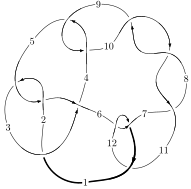
\includegraphics[width=112pt]{../../../GIT/diagram.site/Diagrams/png/833_12a_0032.png}\\
\ \ \ A knot diagram\footnotemark}&
\allowdisplaybreaks
\textbf{Linearized knot diagam} \\
\cline{2-2}
 &
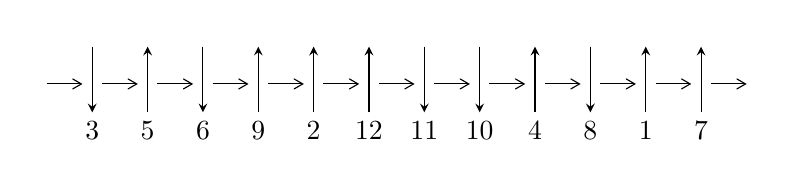
\begin{tikzpicture}[x=20pt, y=17pt]
	% nodes
	\node (C0) at (0, 0) {};
	\node (C1) at (1, 0) {};
	\node (C1U) at (1, +1) {};
	\node (C1D) at (1, -1) {3};

	\node (C2) at (2, 0) {};
	\node (C2U) at (2, +1) {};
	\node (C2D) at (2, -1) {5};

	\node (C3) at (3, 0) {};
	\node (C3U) at (3, +1) {};
	\node (C3D) at (3, -1) {6};

	\node (C4) at (4, 0) {};
	\node (C4U) at (4, +1) {};
	\node (C4D) at (4, -1) {9};

	\node (C5) at (5, 0) {};
	\node (C5U) at (5, +1) {};
	\node (C5D) at (5, -1) {2};

	\node (C6) at (6, 0) {};
	\node (C6U) at (6, +1) {};
	\node (C6D) at (6, -1) {12};

	\node (C7) at (7, 0) {};
	\node (C7U) at (7, +1) {};
	\node (C7D) at (7, -1) {11};

	\node (C8) at (8, 0) {};
	\node (C8U) at (8, +1) {};
	\node (C8D) at (8, -1) {10};

	\node (C9) at (9, 0) {};
	\node (C9U) at (9, +1) {};
	\node (C9D) at (9, -1) {4};

	\node (C10) at (10, 0) {};
	\node (C10U) at (10, +1) {};
	\node (C10D) at (10, -1) {8};

	\node (C11) at (11, 0) {};
	\node (C11U) at (11, +1) {};
	\node (C11D) at (11, -1) {1};

	\node (C12) at (12, 0) {};
	\node (C12U) at (12, +1) {};
	\node (C12D) at (12, -1) {7};
	\node (C13) at (13, 0) {};

	% arrows
	\draw[->,>={angle 60}]
	(C0) edge (C1) (C1) edge (C2) (C2) edge (C3) (C3) edge (C4) (C4) edge (C5) (C5) edge (C6) (C6) edge (C7) (C7) edge (C8) (C8) edge (C9) (C9) edge (C10) (C10) edge (C11) (C11) edge (C12) (C12) edge (C13) ;	\draw[->,>=stealth]
	(C1U) edge (C1D) (C2D) edge (C2U) (C3U) edge (C3D) (C4D) edge (C4U) (C5D) edge (C5U) (C6D) edge (C6U) (C7U) edge (C7D) (C8U) edge (C8D) (C9D) edge (C9U) (C10U) edge (C10D) (C11D) edge (C11U) (C12D) edge (C12U) ;
	\end{tikzpicture} \\
\hhline{~~} \\& 
\textbf{Solving Sequence} \\ \cline{2-2} 
 &
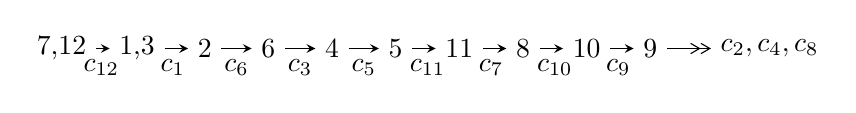
\begin{tikzpicture}[x=23pt, y=7pt]
	% node
	\node (A0) at (-1/8, 0) {7,12};
	\node (A1) at (17/16, 0) {1,3};
	\node (A2) at (17/8, 0) {2};
	\node (A3) at (25/8, 0) {6};
	\node (A4) at (33/8, 0) {4};
	\node (A5) at (41/8, 0) {5};
	\node (A6) at (49/8, 0) {11};
	\node (A7) at (57/8, 0) {8};
	\node (A8) at (65/8, 0) {10};
	\node (A9) at (73/8, 0) {9};
	\node (C1) at (1/2, -1) {$c_{12}$};
	\node (C2) at (13/8, -1) {$c_{1}$};
	\node (C3) at (21/8, -1) {$c_{6}$};
	\node (C4) at (29/8, -1) {$c_{3}$};
	\node (C5) at (37/8, -1) {$c_{5}$};
	\node (C6) at (45/8, -1) {$c_{11}$};
	\node (C7) at (53/8, -1) {$c_{7}$};
	\node (C8) at (61/8, -1) {$c_{10}$};
	\node (C9) at (69/8, -1) {$c_{9}$};
	\node (A10) at (11, 0) {$c_{2},c_{4},c_{8}$};

	% edge
	\draw[->,>=stealth]	
	(A0) edge (A1) (A1) edge (A2) (A2) edge (A3) (A3) edge (A4) (A4) edge (A5) (A5) edge (A6) (A6) edge (A7) (A7) edge (A8) (A8) edge (A9) ;
	\draw[->>,>={angle 60}]	
	(A9) edge (A10);
\end{tikzpicture} \\ 

\end{tabular} \\

\footnotetext{
The image of knot diagram is generated by the software ``\textbf{Draw programme}" developed by Andrew Bartholomew(\url{http://www.layer8.co.uk/maths/draw/index.htm\#Running-draw}), where we modified some parts for our purpose(\url{https://github.com/CATsTAILs/LinksPainter}).
}\phantom \\ \newline 
\centering \textbf{Ideals for irreducible components\footnotemark of $X_{\text{par}}$} 
 
\begin{align*}
I^u_{1}&=\langle 
4 u^{72}+9 u^{71}+\cdots+b-5,\;3 u^{72}+6 u^{71}+\cdots+2 a-5,\;u^{73}+3 u^{72}+\cdots-4 u-1\rangle \\
I^u_{2}&=\langle 
b,\;a^2- a+1,\;u-1\rangle \\
\\
\end{align*}
\raggedright * 2 irreducible components of $\dim_{\mathbb{C}}=0$, with total 75 representations.\\
\footnotetext{All coefficients of polynomials are rational numbers. But the coefficients are sometimes approximated in decimal forms when there is not enough margin.}
\newpage
\renewcommand{\arraystretch}{1}
\centering \section*{I. $I^u_{1}= \langle 4 u^{72}+9 u^{71}+\cdots+b-5,\;3 u^{72}+6 u^{71}+\cdots+2 a-5,\;u^{73}+3 u^{72}+\cdots-4 u-1 \rangle$}
\flushleft \textbf{(i) Arc colorings}\\
\begin{tabular}{m{7pt} m{180pt} m{7pt} m{180pt} }
\flushright $a_{7}=$&$\begin{pmatrix}0\\u\end{pmatrix}$ \\
\flushright $a_{12}=$&$\begin{pmatrix}1\\0\end{pmatrix}$ \\
\flushright $a_{1}=$&$\begin{pmatrix}1\\- u^2\end{pmatrix}$ \\
\flushright $a_{3}=$&$\begin{pmatrix}-\frac{3}{2} u^{72}-3 u^{71}+\cdots+\frac{9}{2} u+\frac{5}{2}\\-4 u^{72}-9 u^{71}+\cdots+14 u+5\end{pmatrix}$ \\
\flushright $a_{2}=$&$\begin{pmatrix}-\frac{1}{2} u^{72}- u^{71}+\cdots-\frac{3}{2} u+\frac{1}{2}\\u^{29}-9 u^{27}+\cdots+2 u^2+u\end{pmatrix}$ \\
\flushright $a_{6}=$&$\begin{pmatrix}- u\\u\end{pmatrix}$ \\
\flushright $a_{4}=$&$\begin{pmatrix}2 u^{72}+5 u^{71}+\cdots-8 u-2\\-\frac{15}{2} u^{72}-17 u^{71}+\cdots+\frac{53}{2} u+\frac{19}{2}\end{pmatrix}$ \\
\flushright $a_{5}=$&$\begin{pmatrix}5 u^{72}+11 u^{71}+\cdots-18 u-6\\\frac{3}{2} u^{72}+3 u^{71}+\cdots-\frac{7}{2} u-\frac{3}{2}\end{pmatrix}$ \\
\flushright $a_{11}=$&$\begin{pmatrix}- u^2+1\\u^4\end{pmatrix}$ \\
\flushright $a_{8}=$&$\begin{pmatrix}- u^5+2 u^3- u\\u^7- u^5+u\end{pmatrix}$ \\
\flushright $a_{10}=$&$\begin{pmatrix}- u^8+3 u^6-3 u^4+1\\u^{10}-2 u^8+u^6+2 u^4- u^2\end{pmatrix}$ \\
\flushright $a_{9}=$&$\begin{pmatrix}- u^{11}+4 u^9-6 u^7+2 u^5+3 u^3-2 u\\u^{13}-3 u^{11}+3 u^9+2 u^7-4 u^5+u^3+u\end{pmatrix}$\\&\end{tabular}
\flushleft \textbf{(ii) Obstruction class $= -1$}\\~\\
\flushleft \textbf{(iii) Cusp Shapes $= -18 u^{72}-43 u^{71}+\cdots+66 u+25$}\\~\\
\newpage\renewcommand{\arraystretch}{1}
\flushleft \textbf{(iv) u-Polynomials at the component}\newline \\
\begin{tabular}{m{50pt}|m{274pt}}
Crossings & \hspace{64pt}u-Polynomials at each crossing \\
\hline $$\begin{aligned}c_{1}\end{aligned}$$&$\begin{aligned}
&u^{73}+32 u^{72}+\cdots+11 u-1
\end{aligned}$\\
\hline $$\begin{aligned}c_{2},c_{5}\end{aligned}$$&$\begin{aligned}
&u^{73}+2 u^{72}+\cdots- u-1
\end{aligned}$\\
\hline $$\begin{aligned}c_{3}\end{aligned}$$&$\begin{aligned}
&u^{73}-2 u^{72}+\cdots+165 u-17
\end{aligned}$\\
\hline $$\begin{aligned}c_{4},c_{9}\end{aligned}$$&$\begin{aligned}
&u^{73}+u^{72}+\cdots+4 u-4
\end{aligned}$\\
\hline $$\begin{aligned}c_{6},c_{12}\end{aligned}$$&$\begin{aligned}
&u^{73}+3 u^{72}+\cdots-4 u-1
\end{aligned}$\\
\hline $$\begin{aligned}c_{7},c_{8},c_{10}\end{aligned}$$&$\begin{aligned}
&u^{73}+15 u^{72}+\cdots-216 u-16
\end{aligned}$\\
\hline $$\begin{aligned}c_{11}\end{aligned}$$&$\begin{aligned}
&u^{73}-43 u^{72}+\cdots-2 u-1
\end{aligned}$\\
\hline
\end{tabular}\\~\\
\newpage\renewcommand{\arraystretch}{1}
\flushleft \textbf{(v) Riley Polynomials at the component}\newline \\
\begin{tabular}{m{50pt}|m{274pt}}
Crossings & \hspace{64pt}Riley Polynomials at each crossing \\
\hline $$\begin{aligned}c_{1}\end{aligned}$$&$\begin{aligned}
&y^{73}+20 y^{72}+\cdots+275 y-1
\end{aligned}$\\
\hline $$\begin{aligned}c_{2},c_{5}\end{aligned}$$&$\begin{aligned}
&y^{73}+32 y^{72}+\cdots+11 y-1
\end{aligned}$\\
\hline $$\begin{aligned}c_{3}\end{aligned}$$&$\begin{aligned}
&y^{73}+8 y^{72}+\cdots-6877 y-289
\end{aligned}$\\
\hline $$\begin{aligned}c_{4},c_{9}\end{aligned}$$&$\begin{aligned}
&y^{73}+15 y^{72}+\cdots-216 y-16
\end{aligned}$\\
\hline $$\begin{aligned}c_{6},c_{12}\end{aligned}$$&$\begin{aligned}
&y^{73}-43 y^{72}+\cdots-2 y-1
\end{aligned}$\\
\hline $$\begin{aligned}c_{7},c_{8},c_{10}\end{aligned}$$&$\begin{aligned}
&y^{73}+83 y^{72}+\cdots+4384 y-256
\end{aligned}$\\
\hline $$\begin{aligned}c_{11}\end{aligned}$$&$\begin{aligned}
&y^{73}-23 y^{72}+\cdots+38 y-1
\end{aligned}$\\
\hline
\end{tabular}\\~\\
\newpage\flushleft \textbf{(vi) Complex Volumes and Cusp Shapes}
$$\begin{array}{c|c|c}  
\text{Solutions to }I^u_{1}& \I (\text{vol} + \sqrt{-1}CS) & \text{Cusp shape}\\
 \hline 
\begin{aligned}
u &= -0.796832 + 0.538347 I \\
a &= -2.31129 + 0.06801 I \\
b &= \phantom{-}1.70540 - 1.05275 I\end{aligned}
 & -4.24142 - 5.70697 I & \phantom{-0.000000 } 0 \\ \hline\begin{aligned}
u &= -0.796832 - 0.538347 I \\
a &= -2.31129 - 0.06801 I \\
b &= \phantom{-}1.70540 + 1.05275 I\end{aligned}
 & -4.24142 + 5.70697 I & \phantom{-0.000000 } 0 \\ \hline\begin{aligned}
u &= \phantom{-}0.899085 + 0.326015 I \\
a &= \phantom{-}0.02535 - 2.32970 I \\
b &= -0.58316 + 2.15466 I\end{aligned}
 & \phantom{-}0.082824 + 0.160201 I & \phantom{-0.000000 } 0 \\ \hline\begin{aligned}
u &= \phantom{-}0.899085 - 0.326015 I \\
a &= \phantom{-}0.02535 + 2.32970 I \\
b &= -0.58316 - 2.15466 I\end{aligned}
 & \phantom{-}0.082824 - 0.160201 I & \phantom{-0.000000 } 0 \\ \hline\begin{aligned}
u &= -1.030080 + 0.324784 I \\
a &= \phantom{-}0.645259 - 0.737289 I \\
b &= \phantom{-}0.428910 - 0.037104 I\end{aligned}
 & \phantom{-}2.50971 + 0.29837 I & \phantom{-0.000000 } 0 \\ \hline\begin{aligned}
u &= -1.030080 - 0.324784 I \\
a &= \phantom{-}0.645259 + 0.737289 I \\
b &= \phantom{-}0.428910 + 0.037104 I\end{aligned}
 & \phantom{-}2.50971 - 0.29837 I & \phantom{-0.000000 } 0 \\ \hline\begin{aligned}
u &= -0.060471 + 0.908501 I \\
a &= -1.143350 + 0.045300 I \\
b &= -0.15329 - 1.46139 I\end{aligned}
 & \phantom{-}6.24864 + 10.27490 I & \phantom{-}2.89542 - 7.01845 I \\ \hline\begin{aligned}
u &= -0.060471 - 0.908501 I \\
a &= -1.143350 - 0.045300 I \\
b &= -0.15329 + 1.46139 I\end{aligned}
 & \phantom{-}6.24864 - 10.27490 I & \phantom{-}2.89542 + 7.01845 I \\ \hline\begin{aligned}
u &= -0.045023 + 0.902001 I \\
a &= \phantom{-}1.048390 - 0.026697 I \\
b &= \phantom{-}0.425897 + 0.828457 I\end{aligned}
 & \phantom{-}8.09212 + 4.88858 I & \phantom{-}5.55498 - 2.56495 I \\ \hline\begin{aligned}
u &= -0.045023 - 0.902001 I \\
a &= \phantom{-}1.048390 + 0.026697 I \\
b &= \phantom{-}0.425897 - 0.828457 I\end{aligned}
 & \phantom{-}8.09212 - 4.88858 I & \phantom{-}5.55498 + 2.56495 I\\
 \hline 
 \end{array}$$\newpage$$\begin{array}{c|c|c}  
\text{Solutions to }I^u_{1}& \I (\text{vol} + \sqrt{-1}CS) & \text{Cusp shape}\\
 \hline 
\begin{aligned}
u &= \phantom{-}1.027830 + 0.411352 I \\
a &= -2.75340 - 1.31041 I \\
b &= \phantom{-}2.13202 + 2.36044 I\end{aligned}
 & \phantom{-}1.86319 + 6.29573 I & \phantom{-0.000000 } 0 \\ \hline\begin{aligned}
u &= \phantom{-}1.027830 - 0.411352 I \\
a &= -2.75340 + 1.31041 I \\
b &= \phantom{-}2.13202 - 2.36044 I\end{aligned}
 & \phantom{-}1.86319 - 6.29573 I & \phantom{-0.000000 } 0 \\ \hline\begin{aligned}
u &= -0.992153 + 0.494153 I \\
a &= -0.13867 + 1.47620 I \\
b &= -0.25797 - 1.67319 I\end{aligned}
 & -2.09315 - 4.25967 I & \phantom{-0.000000 } 0 \\ \hline\begin{aligned}
u &= -0.992153 - 0.494153 I \\
a &= -0.13867 - 1.47620 I \\
b &= -0.25797 + 1.67319 I\end{aligned}
 & -2.09315 + 4.25967 I & \phantom{-0.000000 } 0 \\ \hline\begin{aligned}
u &= -0.003685 + 0.885221 I \\
a &= \phantom{-}1.061200 + 0.001583 I \\
b &= \phantom{-}0.448605 - 0.796552 I\end{aligned}
 & \phantom{-}8.26656 + 1.57314 I & \phantom{-}5.85573 - 2.28832 I \\ \hline\begin{aligned}
u &= -0.003685 - 0.885221 I \\
a &= \phantom{-}1.061200 - 0.001583 I \\
b &= \phantom{-}0.448605 + 0.796552 I\end{aligned}
 & \phantom{-}8.26656 - 1.57314 I & \phantom{-}5.85573 + 2.28832 I \\ \hline\begin{aligned}
u &= \phantom{-}1.061310 + 0.358999 I \\
a &= \phantom{-}1.73187 + 0.46057 I \\
b &= -1.55065 - 1.27425 I\end{aligned}
 & \phantom{-}3.61712 + 1.77427 I & \phantom{-0.000000 } 0 \\ \hline\begin{aligned}
u &= \phantom{-}1.061310 - 0.358999 I \\
a &= \phantom{-}1.73187 - 0.46057 I \\
b &= -1.55065 + 1.27425 I\end{aligned}
 & \phantom{-}3.61712 - 1.77427 I & \phantom{-0.000000 } 0 \\ \hline\begin{aligned}
u &= -1.055210 + 0.377398 I \\
a &= \phantom{-}0.143235 + 0.585101 I \\
b &= -0.653103 + 0.376649 I\end{aligned}
 & \phantom{-}3.48602 - 4.64873 I & \phantom{-0.000000 } 0 \\ \hline\begin{aligned}
u &= -1.055210 - 0.377398 I \\
a &= \phantom{-}0.143235 - 0.585101 I \\
b &= -0.653103 - 0.376649 I\end{aligned}
 & \phantom{-}3.48602 + 4.64873 I & \phantom{-0.000000 } 0\\
 \hline 
 \end{array}$$\newpage$$\begin{array}{c|c|c}  
\text{Solutions to }I^u_{1}& \I (\text{vol} + \sqrt{-1}CS) & \text{Cusp shape}\\
 \hline 
\begin{aligned}
u &= \phantom{-}0.014910 + 0.877594 I \\
a &= -1.170160 + 0.036770 I \\
b &= -0.15465 + 1.42320 I\end{aligned}
 & \phantom{-}6.56651 - 3.81304 I & \phantom{-}3.48761 + 2.37237 I \\ \hline\begin{aligned}
u &= \phantom{-}0.014910 - 0.877594 I \\
a &= -1.170160 - 0.036770 I \\
b &= -0.15465 - 1.42320 I\end{aligned}
 & \phantom{-}6.56651 + 3.81304 I & \phantom{-}3.48761 - 2.37237 I \\ \hline\begin{aligned}
u &= -0.745666 + 0.449141 I \\
a &= \phantom{-}1.241710 - 0.206618 I \\
b &= -0.615729 + 0.808004 I\end{aligned}
 & -1.60556 - 1.91846 I & -0.83992 + 4.54593 I \\ \hline\begin{aligned}
u &= -0.745666 - 0.449141 I \\
a &= \phantom{-}1.241710 + 0.206618 I \\
b &= -0.615729 - 0.808004 I\end{aligned}
 & -1.60556 + 1.91846 I & -0.83992 - 4.54593 I \\ \hline\begin{aligned}
u &= -0.663356 + 0.548451 I \\
a &= -1.09116 + 1.48131 I \\
b &= \phantom{-}0.05851 - 1.82675 I\end{aligned}
 & -4.60806 + 1.34225 I & -6.07081 - 0.60893 I \\ \hline\begin{aligned}
u &= -0.663356 - 0.548451 I \\
a &= -1.09116 - 1.48131 I \\
b &= \phantom{-}0.05851 + 1.82675 I\end{aligned}
 & -4.60806 - 1.34225 I & -6.07081 + 0.60893 I \\ \hline\begin{aligned}
u &= -0.044946 + 0.858380 I \\
a &= -0.926262 - 0.036801 I \\
b &= \phantom{-}0.583114 - 0.035791 I\end{aligned}
 & \phantom{-}2.49214 + 3.07068 I & -0.36042 - 2.48054 I \\ \hline\begin{aligned}
u &= -0.044946 - 0.858380 I \\
a &= -0.926262 + 0.036801 I \\
b &= \phantom{-}0.583114 + 0.035791 I\end{aligned}
 & \phantom{-}2.49214 - 3.07068 I & -0.36042 + 2.48054 I \\ \hline\begin{aligned}
u &= \phantom{-}1.148100 + 0.066282 I \\
a &= \phantom{-}0.481281 - 0.828556 I \\
b &= -0.072635 + 0.333417 I\end{aligned}
 & \phantom{-}0.94991 + 1.54341 I & \phantom{-0.000000 } 0 \\ \hline\begin{aligned}
u &= \phantom{-}1.148100 - 0.066282 I \\
a &= \phantom{-}0.481281 + 0.828556 I \\
b &= -0.072635 - 0.333417 I\end{aligned}
 & \phantom{-}0.94991 - 1.54341 I & \phantom{-0.000000 } 0\\
 \hline 
 \end{array}$$\newpage$$\begin{array}{c|c|c}  
\text{Solutions to }I^u_{1}& \I (\text{vol} + \sqrt{-1}CS) & \text{Cusp shape}\\
 \hline 
\begin{aligned}
u &= \phantom{-}0.831297\phantom{ +0.000000I} \\
a &= \phantom{-}1.18611\phantom{ +0.000000I} \\
b &= -0.878157\phantom{ +0.000000I}\end{aligned}
 & \phantom{-}1.20245\phantom{ +0.000000I} & \phantom{-}8.84780\phantom{ +0.000000I} \\ \hline\begin{aligned}
u &= -1.067090 + 0.480663 I \\
a &= \phantom{-}1.43081 - 0.55418 I \\
b &= -1.10301 + 1.47768 I\end{aligned}
 & \phantom{-}2.23047 - 6.58216 I & \phantom{-0.000000 } 0 \\ \hline\begin{aligned}
u &= -1.067090 - 0.480663 I \\
a &= \phantom{-}1.43081 + 0.55418 I \\
b &= -1.10301 - 1.47768 I\end{aligned}
 & \phantom{-}2.23047 + 6.58216 I & \phantom{-0.000000 } 0 \\ \hline\begin{aligned}
u &= \phantom{-}1.143120 + 0.264741 I \\
a &= \phantom{-}0.321926 - 0.475229 I \\
b &= -0.765191 - 0.174011 I\end{aligned}
 & \phantom{-}3.87826 + 0.47986 I & \phantom{-0.000000 } 0 \\ \hline\begin{aligned}
u &= \phantom{-}1.143120 - 0.264741 I \\
a &= \phantom{-}0.321926 + 0.475229 I \\
b &= -0.765191 + 0.174011 I\end{aligned}
 & \phantom{-}3.87826 - 0.47986 I & \phantom{-0.000000 } 0 \\ \hline\begin{aligned}
u &= -1.072090 + 0.517956 I \\
a &= -2.16667 + 1.15750 I \\
b &= \phantom{-}1.50805 - 2.21750 I\end{aligned}
 & \phantom{-}0.09169 - 11.38030 I & \phantom{-0.000000 } 0 \\ \hline\begin{aligned}
u &= -1.072090 - 0.517956 I \\
a &= -2.16667 - 1.15750 I \\
b &= \phantom{-}1.50805 + 2.21750 I\end{aligned}
 & \phantom{-}0.09169 + 11.38030 I & \phantom{-0.000000 } 0 \\ \hline\begin{aligned}
u &= \phantom{-}1.189960 + 0.217721 I \\
a &= \phantom{-}0.538138 + 0.733544 I \\
b &= \phantom{-}0.386122 - 0.182674 I\end{aligned}
 & \phantom{-}2.38629 - 3.99102 I & \phantom{-0.000000 } 0 \\ \hline\begin{aligned}
u &= \phantom{-}1.189960 - 0.217721 I \\
a &= \phantom{-}0.538138 - 0.733544 I \\
b &= \phantom{-}0.386122 + 0.182674 I\end{aligned}
 & \phantom{-}2.38629 + 3.99102 I & \phantom{-0.000000 } 0 \\ \hline\begin{aligned}
u &= -0.759472 + 0.078072 I \\
a &= \phantom{-}0.409671 + 1.121040 I \\
b &= -0.025028 + 0.368371 I\end{aligned}
 & \phantom{-}0.90189 - 2.32067 I & -2.23029 + 5.61700 I\\
 \hline 
 \end{array}$$\newpage$$\begin{array}{c|c|c}  
\text{Solutions to }I^u_{1}& \I (\text{vol} + \sqrt{-1}CS) & \text{Cusp shape}\\
 \hline 
\begin{aligned}
u &= -0.759472 - 0.078072 I \\
a &= \phantom{-}0.409671 - 1.121040 I \\
b &= -0.025028 - 0.368371 I\end{aligned}
 & \phantom{-}0.90189 + 2.32067 I & -2.23029 - 5.61700 I \\ \hline\begin{aligned}
u &= -0.294691 + 0.697762 I \\
a &= -1.52227 + 0.52821 I \\
b &= \phantom{-}0.04655 - 1.54343 I\end{aligned}
 & -2.13058 + 6.78357 I & -1.78763 - 7.49032 I \\ \hline\begin{aligned}
u &= -0.294691 - 0.697762 I \\
a &= -1.52227 - 0.52821 I \\
b &= \phantom{-}0.04655 + 1.54343 I\end{aligned}
 & -2.13058 - 6.78357 I & -1.78763 + 7.49032 I \\ \hline\begin{aligned}
u &= -0.411090 + 0.594862 I \\
a &= -1.33198 - 0.64422 I \\
b &= \phantom{-}1.058470 - 0.183219 I\end{aligned}
 & -3.71919 - 0.03530 I & -5.73582 - 0.13433 I \\ \hline\begin{aligned}
u &= -0.411090 - 0.594862 I \\
a &= -1.33198 + 0.64422 I \\
b &= \phantom{-}1.058470 + 0.183219 I\end{aligned}
 & -3.71919 + 0.03530 I & -5.73582 + 0.13433 I \\ \hline\begin{aligned}
u &= \phantom{-}0.638508 + 0.276958 I \\
a &= -2.85677 + 1.41704 I \\
b &= \phantom{-}2.23207 - 0.27893 I\end{aligned}
 & -0.67209 + 2.83977 I & \phantom{-}0.57232 - 5.77641 I \\ \hline\begin{aligned}
u &= \phantom{-}0.638508 - 0.276958 I \\
a &= -2.85677 - 1.41704 I \\
b &= \phantom{-}2.23207 + 0.27893 I\end{aligned}
 & -0.67209 - 2.83977 I & \phantom{-}0.57232 + 5.77641 I \\ \hline\begin{aligned}
u &= \phantom{-}1.245740 + 0.440942 I \\
a &= \phantom{-}0.151191 - 1.053990 I \\
b &= -0.087474 + 1.281280 I\end{aligned}
 & \phantom{-}6.38924 + 1.49871 I & \phantom{-0.000000 } 0 \\ \hline\begin{aligned}
u &= \phantom{-}1.245740 - 0.440942 I \\
a &= \phantom{-}0.151191 + 1.053990 I \\
b &= -0.087474 - 1.281280 I\end{aligned}
 & \phantom{-}6.38924 - 1.49871 I & \phantom{-0.000000 } 0 \\ \hline\begin{aligned}
u &= -1.237210 + 0.485257 I \\
a &= \phantom{-}0.092149 + 1.060120 I \\
b &= -0.069199 - 1.349010 I\end{aligned}
 & \phantom{-}6.06816 - 7.90409 I & \phantom{-0.000000 } 0\\
 \hline 
 \end{array}$$\newpage$$\begin{array}{c|c|c}  
\text{Solutions to }I^u_{1}& \I (\text{vol} + \sqrt{-1}CS) & \text{Cusp shape}\\
 \hline 
\begin{aligned}
u &= -1.237210 - 0.485257 I \\
a &= \phantom{-}0.092149 - 1.060120 I \\
b &= -0.069199 + 1.349010 I\end{aligned}
 & \phantom{-}6.06816 + 7.90409 I & \phantom{-0.000000 } 0 \\ \hline\begin{aligned}
u &= -0.247172 + 0.623477 I \\
a &= \phantom{-}1.109370 - 0.156214 I \\
b &= \phantom{-}0.146837 + 0.686540 I\end{aligned}
 & -0.05164 + 2.31958 I & \phantom{-}1.90774 - 3.63180 I \\ \hline\begin{aligned}
u &= -0.247172 - 0.623477 I \\
a &= \phantom{-}1.109370 + 0.156214 I \\
b &= \phantom{-}0.146837 - 0.686540 I\end{aligned}
 & -0.05164 - 2.31958 I & \phantom{-}1.90774 + 3.63180 I \\ \hline\begin{aligned}
u &= -1.254650 + 0.458550 I \\
a &= \phantom{-}0.571192 - 0.618053 I \\
b &= \phantom{-}0.654999 + 0.111159 I\end{aligned}
 & \phantom{-}10.41650 - 0.92595 I & \phantom{-0.000000 } 0 \\ \hline\begin{aligned}
u &= -1.254650 - 0.458550 I \\
a &= \phantom{-}0.571192 + 0.618053 I \\
b &= \phantom{-}0.654999 - 0.111159 I\end{aligned}
 & \phantom{-}10.41650 + 0.92595 I & \phantom{-0.000000 } 0 \\ \hline\begin{aligned}
u &= \phantom{-}1.250410 + 0.474243 I \\
a &= -1.64704 - 1.66951 I \\
b &= \phantom{-}0.99899 + 2.81058 I\end{aligned}
 & \phantom{-}10.30140 + 8.63802 I & \phantom{-0.000000 } 0 \\ \hline\begin{aligned}
u &= \phantom{-}1.250410 - 0.474243 I \\
a &= -1.64704 + 1.66951 I \\
b &= \phantom{-}0.99899 - 2.81058 I\end{aligned}
 & \phantom{-}10.30140 - 8.63802 I & \phantom{-0.000000 } 0 \\ \hline\begin{aligned}
u &= \phantom{-}1.257260 + 0.465604 I \\
a &= \phantom{-}1.34060 + 0.93797 I \\
b &= -1.14852 - 2.06285 I\end{aligned}
 & \phantom{-}12.09550 + 3.22867 I & \phantom{-0.000000 } 0 \\ \hline\begin{aligned}
u &= \phantom{-}1.257260 - 0.465604 I \\
a &= \phantom{-}1.34060 - 0.93797 I \\
b &= -1.14852 + 2.06285 I\end{aligned}
 & \phantom{-}12.09550 - 3.22867 I & \phantom{-0.000000 } 0 \\ \hline\begin{aligned}
u &= -1.256050 + 0.469575 I \\
a &= \phantom{-}0.076133 + 0.366803 I \\
b &= -0.925574 + 0.435365 I\end{aligned}
 & \phantom{-}12.06620 - 6.39600 I & \phantom{-0.000000 } 0\\
 \hline 
 \end{array}$$\newpage$$\begin{array}{c|c|c}  
\text{Solutions to }I^u_{1}& \I (\text{vol} + \sqrt{-1}CS) & \text{Cusp shape}\\
 \hline 
\begin{aligned}
u &= -1.256050 - 0.469575 I \\
a &= \phantom{-}0.076133 - 0.366803 I \\
b &= -0.925574 - 0.435365 I\end{aligned}
 & \phantom{-}12.06620 + 6.39600 I & \phantom{-0.000000 } 0 \\ \hline\begin{aligned}
u &= \phantom{-}1.273530 + 0.443626 I \\
a &= \phantom{-}0.096224 - 0.351788 I \\
b &= -0.940708 - 0.404721 I\end{aligned}
 & \phantom{-}12.14430 - 0.14495 I & \phantom{-0.000000 } 0 \\ \hline\begin{aligned}
u &= \phantom{-}1.273530 - 0.443626 I \\
a &= \phantom{-}0.096224 + 0.351788 I \\
b &= -0.940708 + 0.404721 I\end{aligned}
 & \phantom{-}12.14430 + 0.14495 I & \phantom{-0.000000 } 0 \\ \hline\begin{aligned}
u &= -1.256320 + 0.493887 I \\
a &= \phantom{-}1.29631 - 0.89917 I \\
b &= -1.07374 + 2.03687 I\end{aligned}
 & \phantom{-}11.7702 - 9.8863 I & \phantom{-0.000000 } 0 \\ \hline\begin{aligned}
u &= -1.256320 - 0.493887 I \\
a &= \phantom{-}1.29631 + 0.89917 I \\
b &= -1.07374 - 2.03687 I\end{aligned}
 & \phantom{-}11.7702 + 9.8863 I & \phantom{-0.000000 } 0 \\ \hline\begin{aligned}
u &= \phantom{-}1.279930 + 0.434233 I \\
a &= \phantom{-}0.556079 + 0.623274 I \\
b &= \phantom{-}0.648052 - 0.146041 I\end{aligned}
 & \phantom{-}10.39010 - 5.55528 I & \phantom{-0.000000 } 0 \\ \hline\begin{aligned}
u &= \phantom{-}1.279930 - 0.434233 I \\
a &= \phantom{-}0.556079 - 0.623274 I \\
b &= \phantom{-}0.648052 + 0.146041 I\end{aligned}
 & \phantom{-}10.39010 + 5.55528 I & \phantom{-0.000000 } 0 \\ \hline\begin{aligned}
u &= -1.255820 + 0.502698 I \\
a &= -1.60562 + 1.57330 I \\
b &= \phantom{-}0.94296 - 2.71614 I\end{aligned}
 & \phantom{-}9.8802 - 15.3350 I & \phantom{-0.000000 } 0 \\ \hline\begin{aligned}
u &= -1.255820 - 0.502698 I \\
a &= -1.60562 - 1.57330 I \\
b &= \phantom{-}0.94296 + 2.71614 I\end{aligned}
 & \phantom{-}9.8802 + 15.3350 I & \phantom{-0.000000 } 0 \\ \hline\begin{aligned}
u &= -0.014084 + 0.462153 I \\
a &= \phantom{-}1.42124 + 0.30256 I \\
b &= \phantom{-}0.409463 - 0.530113 I\end{aligned}
 & \phantom{-}0.89929 + 1.38203 I & \phantom{-}4.27247 - 4.11780 I\\
 \hline 
 \end{array}$$\newpage$$\begin{array}{c|c|c}  
\text{Solutions to }I^u_{1}& \I (\text{vol} + \sqrt{-1}CS) & \text{Cusp shape}\\
 \hline 
\begin{aligned}
u &= -0.014084 - 0.462153 I \\
a &= \phantom{-}1.42124 - 0.30256 I \\
b &= \phantom{-}0.409463 + 0.530113 I\end{aligned}
 & \phantom{-}0.89929 - 1.38203 I & \phantom{-}4.27247 + 4.11780 I \\ \hline\begin{aligned}
u &= \phantom{-}0.217836 + 0.395971 I \\
a &= -2.71775 - 0.62754 I \\
b &= \phantom{-}0.30369 + 1.39444 I\end{aligned}
 & -0.21204 - 2.78157 I & \phantom{-}2.07158 + 2.47908 I \\ \hline\begin{aligned}
u &= \phantom{-}0.217836 - 0.395971 I \\
a &= -2.71775 + 0.62754 I \\
b &= \phantom{-}0.30369 - 1.39444 I\end{aligned}
 & -0.21204 + 2.78157 I & \phantom{-}2.07158 - 2.47908 I\\
 \hline 
 \end{array}$$\newpage\newpage\renewcommand{\arraystretch}{1}
\centering \section*{II. $I^u_{2}= \langle b,\;a^2- a+1,\;u-1 \rangle$}
\flushleft \textbf{(i) Arc colorings}\\
\begin{tabular}{m{7pt} m{180pt} m{7pt} m{180pt} }
\flushright $a_{7}=$&$\begin{pmatrix}0\\1\end{pmatrix}$ \\
\flushright $a_{12}=$&$\begin{pmatrix}1\\0\end{pmatrix}$ \\
\flushright $a_{1}=$&$\begin{pmatrix}1\\-1\end{pmatrix}$ \\
\flushright $a_{3}=$&$\begin{pmatrix}a\\0\end{pmatrix}$ \\
\flushright $a_{2}=$&$\begin{pmatrix}a\\-1\end{pmatrix}$ \\
\flushright $a_{6}=$&$\begin{pmatrix}-1\\1\end{pmatrix}$ \\
\flushright $a_{4}=$&$\begin{pmatrix}0\\a\end{pmatrix}$ \\
\flushright $a_{5}=$&$\begin{pmatrix}0\\a\end{pmatrix}$ \\
\flushright $a_{11}=$&$\begin{pmatrix}0\\1\end{pmatrix}$ \\
\flushright $a_{8}=$&$\begin{pmatrix}0\\1\end{pmatrix}$ \\
\flushright $a_{10}=$&$\begin{pmatrix}0\\1\end{pmatrix}$ \\
\flushright $a_{9}=$&$\begin{pmatrix}0\\1\end{pmatrix}$\\&\end{tabular}
\flushleft \textbf{(ii) Obstruction class $= 1$}\\~\\
\flushleft \textbf{(iii) Cusp Shapes $= 4 a+7$}\\~\\
\newpage\renewcommand{\arraystretch}{1}
\flushleft \textbf{(iv) u-Polynomials at the component}\newline \\
\begin{tabular}{m{50pt}|m{274pt}}
Crossings & \hspace{64pt}u-Polynomials at each crossing \\
\hline $$\begin{aligned}c_{1},c_{3},c_{5}\end{aligned}$$&$\begin{aligned}
&u^2- u+1
\end{aligned}$\\
\hline $$\begin{aligned}c_{2}\end{aligned}$$&$\begin{aligned}
&u^2+u+1
\end{aligned}$\\
\hline $$\begin{aligned}c_{4},c_{7},c_{8}\\c_{9},c_{10}\end{aligned}$$&$\begin{aligned}
&u^2
\end{aligned}$\\
\hline $$\begin{aligned}c_{6},c_{11}\end{aligned}$$&$\begin{aligned}
&(u+1)^2
\end{aligned}$\\
\hline $$\begin{aligned}c_{12}\end{aligned}$$&$\begin{aligned}
&(u-1)^2
\end{aligned}$\\
\hline
\end{tabular}\\~\\
\newpage\renewcommand{\arraystretch}{1}
\flushleft \textbf{(v) Riley Polynomials at the component}\newline \\
\begin{tabular}{m{50pt}|m{274pt}}
Crossings & \hspace{64pt}Riley Polynomials at each crossing \\
\hline $$\begin{aligned}c_{1},c_{2},c_{3}\\c_{5}\end{aligned}$$&$\begin{aligned}
&y^2+y+1
\end{aligned}$\\
\hline $$\begin{aligned}c_{4},c_{7},c_{8}\\c_{9},c_{10}\end{aligned}$$&$\begin{aligned}
&y^2
\end{aligned}$\\
\hline $$\begin{aligned}c_{6},c_{11},c_{12}\end{aligned}$$&$\begin{aligned}
&(y-1)^2
\end{aligned}$\\
\hline
\end{tabular}\\~\\
\newpage\flushleft \textbf{(vi) Complex Volumes and Cusp Shapes}
$$\begin{array}{c|c|c}  
\text{Solutions to }I^u_{2}& \I (\text{vol} + \sqrt{-1}CS) & \text{Cusp shape}\\
 \hline 
\begin{aligned}
u &= \phantom{-}1.00000\phantom{ +0.000000I} \\
a &= \phantom{-}0.500000 + 0.866025 I \\
b &= \phantom{-0.000000 } 0\end{aligned}
 & \phantom{-}1.64493 - 2.02988 I & \phantom{-}9.00000 + 3.46410 I \\ \hline\begin{aligned}
u &= \phantom{-}1.00000\phantom{ +0.000000I} \\
a &= \phantom{-}0.500000 - 0.866025 I \\
b &= \phantom{-0.000000 } 0\end{aligned}
 & \phantom{-}1.64493 + 2.02988 I & \phantom{-}9.00000 - 3.46410 I\\
 \hline 
 \end{array}$$\newpage
\newpage\renewcommand{\arraystretch}{1}
\centering \section*{ III. u-Polynomials}
\begin{tabular}{m{50pt}|m{274pt}}
Crossings & \hspace{64pt}u-Polynomials at each crossing \\
\hline $$\begin{aligned}c_{1}\end{aligned}$$&$\begin{aligned}
&(u^2- u+1)(u^{73}+32 u^{72}+\cdots+11 u-1)
\end{aligned}$\\
\hline $$\begin{aligned}c_{2}\end{aligned}$$&$\begin{aligned}
&(u^2+u+1)(u^{73}+2 u^{72}+\cdots- u-1)
\end{aligned}$\\
\hline $$\begin{aligned}c_{3}\end{aligned}$$&$\begin{aligned}
&(u^2- u+1)(u^{73}-2 u^{72}+\cdots+165 u-17)
\end{aligned}$\\
\hline $$\begin{aligned}c_{4},c_{9}\end{aligned}$$&$\begin{aligned}
&u^2(u^{73}+u^{72}+\cdots+4 u-4)
\end{aligned}$\\
\hline $$\begin{aligned}c_{5}\end{aligned}$$&$\begin{aligned}
&(u^2- u+1)(u^{73}+2 u^{72}+\cdots- u-1)
\end{aligned}$\\
\hline $$\begin{aligned}c_{6}\end{aligned}$$&$\begin{aligned}
&((u+1)^2)(u^{73}+3 u^{72}+\cdots-4 u-1)
\end{aligned}$\\
\hline $$\begin{aligned}c_{7},c_{8},c_{10}\end{aligned}$$&$\begin{aligned}
&u^2(u^{73}+15 u^{72}+\cdots-216 u-16)
\end{aligned}$\\
\hline $$\begin{aligned}c_{11}\end{aligned}$$&$\begin{aligned}
&((u+1)^2)(u^{73}-43 u^{72}+\cdots-2 u-1)
\end{aligned}$\\
\hline $$\begin{aligned}c_{12}\end{aligned}$$&$\begin{aligned}
&((u-1)^2)(u^{73}+3 u^{72}+\cdots-4 u-1)
\end{aligned}$\\
\hline
\end{tabular}\newpage\renewcommand{\arraystretch}{1}
\centering \section*{ IV. Riley Polynomials}
\begin{tabular}{m{50pt}|m{274pt}}
Crossings & \hspace{64pt}Riley Polynomials at each crossing \\
\hline $$\begin{aligned}c_{1}\end{aligned}$$&$\begin{aligned}
&(y^2+y+1)(y^{73}+20 y^{72}+\cdots+275 y-1)
\end{aligned}$\\
\hline $$\begin{aligned}c_{2},c_{5}\end{aligned}$$&$\begin{aligned}
&(y^2+y+1)(y^{73}+32 y^{72}+\cdots+11 y-1)
\end{aligned}$\\
\hline $$\begin{aligned}c_{3}\end{aligned}$$&$\begin{aligned}
&(y^2+y+1)(y^{73}+8 y^{72}+\cdots-6877 y-289)
\end{aligned}$\\
\hline $$\begin{aligned}c_{4},c_{9}\end{aligned}$$&$\begin{aligned}
&y^2(y^{73}+15 y^{72}+\cdots-216 y-16)
\end{aligned}$\\
\hline $$\begin{aligned}c_{6},c_{12}\end{aligned}$$&$\begin{aligned}
&((y-1)^2)(y^{73}-43 y^{72}+\cdots-2 y-1)
\end{aligned}$\\
\hline $$\begin{aligned}c_{7},c_{8},c_{10}\end{aligned}$$&$\begin{aligned}
&y^2(y^{73}+83 y^{72}+\cdots+4384 y-256)
\end{aligned}$\\
\hline $$\begin{aligned}c_{11}\end{aligned}$$&$\begin{aligned}
&((y-1)^2)(y^{73}-23 y^{72}+\cdots+38 y-1)
\end{aligned}$\\
\hline
\end{tabular}
\vskip 2pc
\end{document}